\centering
\begin{minipage}[t]{0.48\textwidth}
\centering\textbf{A\quad Validation outcomes}\par\vspace{0.9cm}
\small\begin{tabular}{lrr}
\toprule Class & Captured & Crossed arm \\
\midrule Downward & $1024/1024$ & $0$ \\
Moving & $1024/1024$ & $6$ \\
Near upright & $1024/1024$ & $0$ \\
Tight upright & $1024/1024$ & $0$ \\
\midrule Fixed probes & $8/8$ & $0$ \\
\bottomrule
\end{tabular}\par\vspace{0.7cm}
{\footnotesize Capture and containment are separate outcomes.}
\end{minipage}\hfill
\begin{minipage}[t]{0.49\textwidth}
\centering\textbf{B\quad Capture-time distributions}\par
\begin{tikzpicture}\begin{axis}[width=\linewidth,height=4.8cm,
 xlabel={Capture time (s)},ylabel={Cumulative fraction},xmin=0,xmax=20,ymin=0,ymax=1.03,
 legend pos=south east,legend cell align=left]
\addplot[armblue,const plot] coordinates {\DownCdf};\addlegendentry{Downward}
\addplot[pendorange,const plot] coordinates {\MovingCdf};\addlegendentry{Moving}
\addplot[energygreen,const plot] coordinates {\NearCdf};\addlegendentry{Near upright}
\addplot[curvepurple,dashed,const plot] coordinates {\TightCdf};\addlegendentry{Tight upright}
\end{axis}\end{tikzpicture}
\end{minipage}
\par\vspace{0.55cm}
\begin{minipage}[t]{0.48\textwidth}
\centering\textbf{C\quad Median-time downward replay}\par
\begin{tikzpicture}\begin{axis}[width=\linewidth,height=4.05cm,
 ylabel={Angle ($^\circ$)},xmin=0,xmax=11.12,ymin=-100,ymax=370,
 xticklabels=\empty,ytick={0,180,360},unbounded coords=jump,legend columns=2,
 legend style={at={(0.5,1.04)},anchor=south}]
\addplot[draw=none,fill=energygreen!15,forget plot] coordinates {(0,165)(11.12,165)(11.12,195)(0,195)}--cycle;
\addplot[armblue] coordinates {\MedianArm};\addlegendentry{$\theta$}
\addplot[pendorange] coordinates {\MedianPend};\addlegendentry{$\alpha$}
\end{axis}\end{tikzpicture}\par\vspace{-0.25cm}
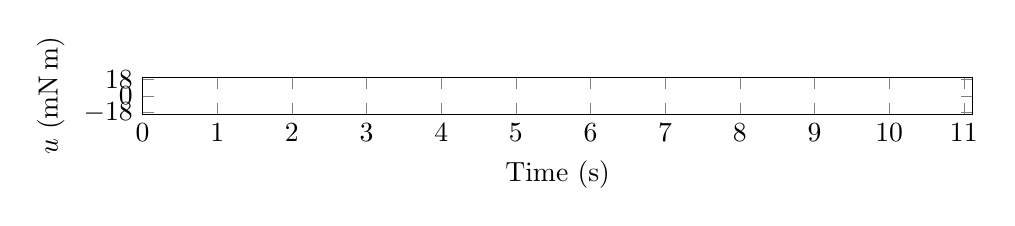
\begin{tikzpicture}\begin{axis}[width=\linewidth,height=2.05cm,
 xlabel={Time (s)},ylabel={$u$ (mN\,m)},xmin=0,xmax=11.12,ymin=-20,ymax=20,ytick={-18,0,18}]
\addplot[black,const plot mark right,thin] coordinates {\MedianTorque};
\end{axis}\end{tikzpicture}
\end{minipage}\hfill
\begin{minipage}[t]{0.49\textwidth}
\centering\textbf{D\quad Physical energy components}\par
\begin{tikzpicture}\begin{axis}[width=\linewidth,height=5.85cm,
 xlabel={Time (s)},ylabel={Energy (mJ)},xmin=0,xmax=11.12,ymin=0,ymax=35,
 legend columns=2,legend style={at={(0.5,1.04)},anchor=south}]
\addplot[armblue] coordinates {\MedianKa};\addlegendentry{$K_a$}
\addplot[curvepurple] coordinates {\MedianKp};\addlegendentry{$K_p$}
\addplot[energygreen] coordinates {\MedianV};\addlegendentry{$V$}
\addplot[black] coordinates {\MedianE};\addlegendentry{$E$}
\addplot[gray,dashed] coordinates {(0,30.37176)(11.12,30.37176)};
\node[anchor=south east,font=\scriptsize,fill=white] at (axis cs:11.1,30.37176){$E_\star$};
\end{axis}\end{tikzpicture}
\end{minipage}
\par\vspace{0.55cm}
\begin{minipage}[t]{0.48\textwidth}
\centering\textbf{E\quad Slow downward replay}\par
\begin{tikzpicture}\begin{axis}[width=\linewidth,height=4.6cm,
 xlabel={Time (s)},ylabel={Angle ($^\circ$)},xmin=0,xmax=16.92,ymin=-100,ymax=370,
 ytick={0,180,360},unbounded coords=jump]
\addplot[draw=none,fill=energygreen!15,forget plot] coordinates {(0,165)(16.92,165)(16.92,195)(0,195)}--cycle;
\addplot[armblue] coordinates {\SlowArm};
\addplot[pendorange] coordinates {\SlowPend};
\end{axis}\end{tikzpicture}
\end{minipage}\hfill
\begin{minipage}[t]{0.49\textwidth}
\centering\textbf{F\quad First arm crossings}\par
\begin{tikzpicture}\begin{axis}[width=\linewidth,height=4.6cm,
 xlabel={Time from first crossing (s)},ylabel={$|\theta|$ ($^\circ$)},xmin=-1.2,xmax=1.2,ymin=100,ymax=195,
 legend pos=south east,legend cell align=left]
\addplot[curvepurple] coordinates {\CrossBounded};\addlegendentry{Bounded options existed}
\addplot[pendorange] coordinates {\CrossUnbounded};\addlegendentry{No bounded tested option}
\addplot[black,dashed] coordinates {(-1.2,180)(1.2,180)};
\addplot[gray,dotted] coordinates {(0,100)(0,195)};
\end{axis}\end{tikzpicture}
\end{minipage}
